\section{Tensor Derivatives: levelling up the rizz!}
Till now, we had just seen the transformation of tensors and tensor densities. However, an important aspect of any calculation is the ability to take derivatives \footnote{A person's intellectual prowess can be judged their ability to take derivatives \emoji{smiling-face-with-sunglasses}}. Derivatives occur everywhere in calculations and we need a way to tackle them. So let's start\dots

\subsection{Velocity}
Well velocity is a vector (we had been reminded many a times) and it should then transform as a vector. Now, 
we know the transformation:
$$dx'^i = \pdv{x'^i}{x^l}x^l$$
To find velocity components, we have to differentiate with respect to time $t$. 
\begin{align*}
    \dv{x'^i}{t} &= \dv{t}\brac{\pdv{x'^i}{x^l}x^l}\\
    &=\pdv{x'^i}{x^l}\dv{x^l}{t} + x^l \dv{t}\brac{\pdv{x'^i}{x^l}}\\
    &=\pdv{x'^i}{x^l}\dv{x^l}{t} + x^l \pdv{x'^i}{x^k}{x^l}\dv{x^k}{t}
\end{align*}
Now we define $v^k = \dv{x^k}{t}$. Then the above expression would give:
\begin{align*}
    v'^i = \pdv{x'^i}{x^l}v^l +  \pdv{x'^i}{x^k}{x^l}x^l v^k
\end{align*}
The first term gives the proper thing for velocity to be a vector, like the correct transformation. The second term is the BAD term \emoji{face-with-steam-from-nose}. Let's see some examples of this term in some transformation:\\[0.3cm]
\textbf{Rotation:}
\begin{align*}
    x' &= x\cos\theta+y\sin\theta\\
    y'&=-x\sin\theta + y\cos\theta
\end{align*}
So we have: 
\begin{align*}
    \pdv{x'}{x} = \cos\theta \quad  \pdv{x'}{y} = \sin\theta \quad  \pdv{y'}{x} = -\sin\theta \quad
    \pdv{y'}{y} = \cos\theta
\end{align*}
Note that the first derivatives do not depend on the coordinate anymore. For a fixed $\theta$, the first derivatives are constants. 
And if we consider the transformation of the velocity components, then the second term will vanish, since these contain double derivatives. Thus, the BAD term vanishes and we happily see that velocity is a vector under rotation. In Galilean transformation ($x'=x-vt, y'=y, z'=z, t'=t$) too, the second term vanish. Even in Lorentz transformation ($t' = \gamma \brac{t-vx}, x=\gamma(x-vt), y'=y, z'=z$) the bad term vanishes. So in basic transformations, velocity is indeed a vector. Let us now see how derivative of a tensor component transforms. So we have,
\begin{align*}
    (\partial_\lambda T^\alpha)' = \partial_{\lambda'}\mathcolor{red}{T'^\lambda}&= \mathcolor{blue}{\frac{\partial}{\partial x'^\lambda}}\brac{\mathcolor{red}{\pdv{x'\lambda}{x^\sigma}T^\sigma}} \quad \ \ (\text{contravariant transformation of tensor})\\
    &= \mathcolor{blue}{\pdv{x^\rho}{x'^\lambda}\frac{\partial}{\partial x^\rho}}\brac{{\pdv{x'^\lambda}{x^\sigma}T^\sigma}}\quad \ \ (\text{covariant transformation of derivative})\\
    &= \pdv{x^\rho}{x'^\lambda}\pdv{x'^\alpha}{x^\sigma}\partial_\rho T^\sigma + \pdv{x^\rho}{x'^\lambda}\pdv{x'^\alpha}{x^\rho}{x^\sigma}T^\sigma \quad \ \ (\text{chain rule})
\end{align*}
Again, the first term is the usual thing but the BAD term appears again! Notice how always the bad term contains a double derivative. Now we know that double derivatives have something to do with curvatures. Let us clarify a bit more.\\[0.3cm]
Imagine the position vector $\veb{r}(t)$ on a flat space. Then the tangent vector to a point having position $\veb{r}(t)$, say $\veb{v}$, will lie entirely on the same space, right? But now, imagine the space being curved. Now if we draw the tangent, it will inevitable leave the space. Imagine the people living on the surface of a sphere. The velocity vector for a moving body in the space will be tangent to the sphere and points off of it. So, for the inhabitants, the velocity vector doesn't exist since it is not contained entirely on the space (Is this the same case with \textit{God}? Hmm, something to think about \emoji{thinking}). What they can do it, just take some small patch of the sphere (which is flat) where the tangent touches the surface and around it, locally, they can define the velocity vector. So, in general the velocity is not a tensor in curved space, where the second derivative is non-zero. 

% \begin{figure}[H]
%     \centering 
%     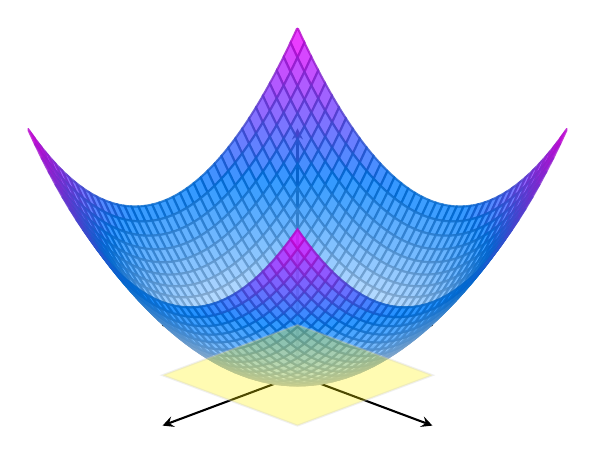
\begin{tikzpicture}
  \begin{axis}[
      view={135}{30},
      colormap/cool,
      axis lines=center,
      xlabel={}, ylabel={}, zlabel={},
      domain=-2:2,
      y domain=-2:2,
      samples=40,
      samples y=40,xtick=\empty,
ytick=\empty,
ztick=\empty
    ]

    % Paraboloid surface z = x^2 + y^2
    \addplot3[
      surf,
      opacity=0.8
    ]
    {x^2 + y^2};

    % Tangent plane at origin z = 0
    \addplot3 [
      surf,
      domain=-1:1,
      y domain=-1:1,
      samples=2,
      samples y=2,
      fill=yellow,
      opacity=0.3
    ]
    {0};

  
   

  \end{axis}
\end{tikzpicture}
%     \caption{Notice how all the tangents at the lowest point of the paraboloid $(x=0,y=0)$ is constrained to be in the yellow coloured plane. Now only some area around $x=0,y=0$ can be made to look locally like the yellow plane and hence the definition of velocity will be valid only locally, within that patch.   }
% \end{figure}
\subsection{Affine Connection}
Suppose in a locally inertial frame, for an object we have zero acceleration, that is:
$$\dv[2]{X^\alpha}{\uptau} = 0$$
Suppose the coordinates $X^\alpha \equiv X^\alpha(x^\mu)$ where $x^\mu$ are coordinates of a ground-based inertial reference frame relative to which the object accelerates. Then using chain rule, we have from the previous relation:
$$\frac{d}{d\uptau}\brac{\pdv{X^\alpha}{x^\mu}\dv{x^\mu}{\uptau}} = 0$$

Using product rule and chain rule again, we have:
$$\pdv{X^\alpha}{x^\mu}\dv[2]{x^\mu}{\uptau} +\pdv{X^\alpha}{x^\mu}{x^\rho} \dv{x^\rho}{\uptau} \dv{x^\mu}{\uptau}=0$$
Now we do one nice thing: multiply the above with $\pdv{x^\lambda}{X^\alpha}$:
$$\pdv{x^\lambda}{X^\alpha}\brac{\pdv{X^\alpha}{x^\mu}\dv[2]{x^\mu}{\uptau}} +\pdv{x^\lambda}{X^\alpha}\brac{\pdv{X^\alpha}{x^\mu}{x^\rho} \dv{x^\rho}{\uptau} \dv{x^\mu}{\uptau}}=0$$
Doing this, a nice thing occurs but for that we have to note that $\pdv{x^\lambda}{X^\alpha}\pdv{X^\alpha}{X^\mu} = \tensor{\delta}{^\lambda _\mu}$. Then from the first term, we get the kronecker delta and the expression reduces to:
$$\dv[2]{x^\lambda}{\uptau} +\mathcolor{blue}{\pdv{x^\lambda}{X^\alpha}\pdv{X^\alpha}{x^\mu}{x^\rho}} \dv{x^\rho}{\uptau} \dv{x^\mu}{\uptau}=0 \quad \implies \quad \dv[2]{x^\lambda}{\uptau} +\mathcolor{blue}{\tensor{\Gamma}{^\lambda _\mu _\rho}} \dv{x^\rho}{\uptau} \dv{x^\mu}{\uptau}=0$$
Here we have identified the scary blue term with a symbol with three indices, one upper and two lower (since in the blue term, there is one upper and two lower indices). This thing, we call the \textbf{affine connection}. 
Note that since derivatives commute\footnote{If a space has something called a `torsion', then the derivatives no longer commute and the following property does not hold true} generally, we have the lower indices of the affine connection to be symmetric, that is,
$$\tensor{\Gamma}{^\alpha _\mu _\nu} =\tensor{\Gamma}{^\alpha _\nu _\mu}$$
\subsubsection{Definition in terms of basis vectors}
We can define the affine connection using basis vectors also. Consider the derivative of the basis vector $\veb{e}_i$ with respect to some coordinates. This derivate is another vector which when expanded in terms of the basis, the coefficients are nothing but the affine connection. 
$$\pdv{\veb{e}_i}{x^j} = \tensor{\Gamma}{^k _{ij}}\veb{e}_k$$

\subsubsection{Transformation of Affine Connection}
Note that the affine connection contains both coordinates $X^\alpha$ and $x\mu$. Suppose we want to transform from $x$ to $x'$ coordinate system, then only the $x$ things will be changed, not the $X$ things. Leave the $X$ alone because the transformation being studied is specifically about how the connection coefficients behave when you change coordinate systems on the ground. So we have:
\begin{align*}
    \tensor{(\Gamma')}{^\lambda _\mu _\nu} &= \mathcolor{blue}{\pdv{x'^\lambda}{X^\alpha}}\pdv{X^\alpha}{x'^\mu}{x'^\nu}\\
    &= \mathcolor{blue}{\pdv{x'^\lambda}{x^\rho}\pdv{x^\rho}{X^\alpha}}\pdv{X^\alpha}{x'^\mu}{x'^\nu} \quad \text{(using chain rule )}\\
    &=\brac{\pdv{x'^\lambda}{x^\rho}\pdv{x^\rho}{X^\alpha}} \pdv{x'^\mu}\brac{\mathcolor{OliveGreen}{\pdv{X^\alpha}{x^\sigma}}\mathcolor{red}{ \pdv{x^\sigma}{x'^\nu}}} \quad \text{(using chain rule again )}\\
    &=\brac{\pdv{x'^\lambda}{x^\rho}\pdv{x^\rho}{X^\alpha}}\brac{ { \mathcolor{red}{\pdv{x^\sigma}{x'^\nu}}\pdv{x'^\mu}\brac{\mathcolor{OliveGreen}{\pdv{X^\alpha}{x^\sigma}}} + \mathcolor{OliveGreen}{\pdv{X^\alpha}{x^\sigma}}\pdv{\mathcolor{red}{x^\sigma}}{x'^\mu}{\mathcolor{red}{x'^\nu}}}}\quad \text{(using product rule )}\\
    &=\brac{\pdv{x'^\lambda}{x^\rho}\pdv{x^\rho}{X^\alpha}} \brac{\pdv{x^\sigma}{x'^\nu} \pdv{X^\alpha}{x^\kappa}{x^\sigma}\pdv{x^\kappa}{x'^\mu}+ \pdv{X^\alpha}{x^\sigma}\pdv{x^\sigma}{x'^\mu}{x'^\nu}}\quad \text{(using chain rule )}
\end{align*}
Well well, I know this was a shitty calculation but hey, sometimes shit is what relieves us! We now focus on the two terms separately in the above expression. 
\begin{itemize}
    \item \textbf{The First Term:} $\brac{\pdv{x'^\lambda}{x^\rho}\pdv{x^\rho}{X^\alpha}}\pdv{x^\sigma}{x'^\nu} \pdv{X^\alpha}{x^\kappa}{x^\sigma}\pdv{x^\kappa}{x'^\mu}$\\[0.3cm]
This can be rearranged a bit and can be written as 
$$   \brac{\pdv{x'^\lambda}{x^\rho}\pdv{x^\sigma}{x'^\nu} \pdv{x^\kappa}{x'^\mu}}   \brac{\pdv{x^\rho}{X^\alpha}\pdv{X^\alpha}{x^\kappa}{x^\sigma}} \equiv \brac{\pdv{x'^\lambda}{x^\rho}\pdv{x^\sigma}{x'^\nu} \pdv{x^\kappa}{x'^\mu}}  \tensor{\Gamma}{^\rho _\kappa _\sigma}$$
\item \textbf{The Second Term:} $\brac{\pdv{x'^\lambda}{x^\rho}\mathcolor{blue}{\pdv{x^\rho}{X^\alpha}}}\mathcolor{blue}{\pdv{X^\alpha}{x^\sigma}}\pdv{x^\sigma}{x'^\mu}{x'^\nu}$
The blue terms together gives $\tensor{\delta}{^\rho _\sigma}$ which reduces the expression to:
$$\pdv{x'^\lambda}{x^\rho}\pdv{x^\rho}{x'^\mu}{x'^\nu}$$
\end{itemize}
Thus, finally we obtain the expression for the transformation of the affine connection:
$$\boxed{ \tensor{(\Gamma')}{^\lambda _\mu _\nu} = \brac{\pdv{x'^\lambda}{x^\rho}\pdv{x^\sigma}{x'^\nu} \pdv{x^\kappa}{x'^\mu}}  \tensor{\Gamma}{^\rho _\kappa _\sigma} +\pdv{x'^\lambda}{x^\rho}\pdv{x^\rho}{x'^\mu}{x'^\nu} }$$
Note that the first term is the usual transformation rule for the affine connection but again the second BAD term emerges which, if non-zero, will lead to the affine connection not being a tensor.\\[0.3cm]
Now note that the BAD term contains the second derivative of the old coordinates with respect to the old coordinates, but generally we have the other way. So it would be a bit nice if we could change it. For that, note the identity and differentiate with respect to $x'^\mu$:
\begin{align*}
   &\pdv{x'^\lambda}{x^\rho}\pdv{x^\rho}{x'^\nu}=\tensor{\delta}{^\lambda_\nu}\\
\implies & \pdv{x'^\mu}\brac{\pdv{x'^\lambda}{x^\rho}\pdv{x^\rho}{x'^\nu}}=0\\
\implies & \brac{\pdv{x'^\lambda}{x^\rho}} \brac{\pdv{x^\rho}{x'^\nu}{x'^\mu} }+ \brac{\pdv{x^\rho}{x'^\nu}}\brac{\pdv{x'^\lambda}{x^\rho}{x'^\mu}}=0\\
\implies & \brac{\pdv{x'^\lambda}{x^\rho}} \brac{\pdv{x^\rho}{x'^\nu}{x'^\mu} } + \brac{\pdv{x^\rho}{x'^\nu}}\brac{\pdv{x'^\lambda}{x^\rho}{x^\sigma}\pdv{x^\sigma}{x'^\mu}}=0
\end{align*}
The first term in the above is exactly the BAD term in the affine connection transformation and thus we replace this. Then we have: 
$$\boxed{ \tensor{(\Gamma')}{^\lambda _\mu _\nu} = \brac{\pdv{x'^\lambda}{x^\rho}\pdv{x^\sigma}{x'^\nu} \pdv{x^\kappa}{x'^\mu}}  \tensor{\Gamma}{^\rho _\kappa _\sigma} - \brac{\pdv{x^\rho}{x'^\nu}}\brac{\pdv{x'^\lambda}{x^\rho}{x^\sigma}\pdv{x^\sigma}{x'^\mu}} }$$
\subsection{Covariant Derivatives}
In every transformation seen so far, we had got a BAD term (containing a second derivative) which spoils the transformation. So wouldn't it be nice if we just redefine the definition of a derivative so that this BAD term gets cancelled from the definition only? This brings us to \textit{covariant derivative} 
\\[0.3cm]
\textbf{A Notational Nightmare:}\\[0.3cm]
The symbol of covariant derivative is very confusing. Different people use different notation for it. Some use $D$ for it, some use $\nabla$ while some use $;$. We will use $;$ for it, I guess but we may sometimes shift to $D$ notation if ambiguity arises...\\[0.3cm]
The covariant derivative of a vector component with respect to a scalar is defined as:
$$\frac{DA^\lambda}{D\uptau} := \frac{dA^\lambda}{d\uptau}+ \tensor{\Gamma}{^\lambda _\mu _\nu}\dv{x^\mu}{\uptau}A^\nu$$
Here we used the $D$ notation since the $;$ notation is mostly used when we differentiate with respect to some coordinate. The covariant derivative of a vector component with respect to a coordinate is then\footnote{$\tensor{A}{^\nu _, _\mu}$ means the normal derivative, that is, $\partial_\mu A^\nu$}: 
$$\tensor{A}{^\lambda _; _\mu} :=  \tensor{A}{^\lambda _, _\mu} +\tensor{\Gamma}{^\lambda _\mu _\nu}A^\nu$$
The covariant derivative of a covariant component is similarly defined:
$$\tensor{A}{_\lambda _; _\mu} :=  \tensor{A}{_\lambda _, _\mu} +\tensor{\Gamma}{^\alpha _\lambda _\nu}A_\alpha$$
\subsubsection{Transformation of Covariant Derivative}
In the primed frame, we have: 
\begin{align*}
\tensor{{A'}}{^\lambda _{;\uptau}} &= \tensor{{A'}}{^\lambda _{,\uptau}} + \tensor{{\Gamma'}}{^\lambda _{\mu \nu}} \dv{x'^\mu}{\uptau} \tensor{{A'}}{^\nu} \\
&= \left( \pdv{x'^\lambda}{x^l} \dv{A^l}{\uptau} 
+ A^l \pdv{x'^\lambda}{x^k}{x^l} \dv{x^k}{\uptau} \right) \\
&\quad + \Bigg[ 
\brac{\pdv{x'^\lambda}{x^\rho}\pdv{{x^\sigma}}{{x'^\nu}} \pdv{{x^\kappa}}{{x'^\mu}}}  \tensor{\Gamma}{^\rho _\kappa _\sigma} - \brac{\pdv{{x^\rho}}{{x'^\nu}}}\brac{\pdv{x'^\lambda}{x^\rho}{x^\sigma}\pdv{{x^\sigma}}{{x'^\mu}}}  \Bigg]
 \\
&\qquad \times \left( 
\pdv{x'^\mu}{x^\omega} \dv{x^\omega}{\uptau} 
+ x^\omega \pdv[2]{x'^\mu}{x^\omega}{x^\beta} \dv{x^\beta}{\uptau} 
\right)
\pdv{{x'^\nu}}{{x^\theta}} A^\theta
\end{align*}
Let's see this term by term. 
\begin{itemize}
    \item \textbf{The First Term:} Transformation of normal derivative 
    $$ \boxed{\pdv{x'^\lambda}{x^l} \dv{A^l}{\uptau} }
+ \mathcolor{OliveGreen}{A^l \pdv{x'^\lambda}{x^q}{x^l} \dv{x^q}{\uptau}}$$
This is fine for now. Let's leave it here!
    \item \textbf{The Second Term:} Multiplication of three individual terms
    Well, this is the monster \emoji{alien-monster} actually. When expanded, it will have four terms. Let us write them one by one: 
    \begin{enumerate}
        \item After reducing the Kronecker delta, the final expression becomes: \begin{align*} 
            \pdv{x'^\lambda}{x^\rho}\pdv{{x^\sigma}}{\mathcolor{blue}{x'^\nu}} \pdv{{x^\kappa}}{\mathcolor{purple}{x'^\mu}}\pdv{\mathcolor{blue}{x'^\nu}}{x^\theta}\pdv{\mathcolor{purple}{x'^\mu}}{x^\omega}\dv{x^\omega}{\uptau}\tensor{\Gamma}{^\rho _\kappa _\sigma}A^\theta =\boxed{\pdv{x'^\lambda}{x^\rho}\dv{x^\kappa}{\uptau}\tensor{\Gamma}{^\rho _\kappa _\sigma}A^\sigma}
        \end{align*}
        \item After reducing the Kronecker delta, we have:
        \begin{align*}
            - {\pdv{{x^\rho}}{\mathcolor{blue}{x'^\nu}}}{\pdv{x'^\lambda}{x^\rho}{x^\sigma}\pdv{{x^\sigma}}{{\mathcolor{red}{{x'^\mu}}}}}\pdv{\mathcolor{blue}{x'^\nu}}{x^\theta}\pdv{\mathcolor{red}{x'^\mu}}{x^\omega}\dv{x^\omega}{\uptau}A^\theta = -\mathcolor{OliveGreen}{\pdv{x'^\lambda}{x^\rho}{x^\sigma} \dv{x^\sigma}{\uptau}A^\rho}
        \end{align*}
        Note this final term and the \textbf{first term}, both of these differ only by the fact that $q\rightarrow \sigma$ and $l \rightarrow \rho$ but since these are dummy indices, we can just rename them and these terms are actually equal but we have a minus sign in this term, so this cancels with the first term. 
        \item After reducing the Kronecker delta, we have:
        \begin{align*}
            \pdv{x'^\lambda}{x^\rho} \pdv{x^\kappa}{x'^\mu} \pdv{x'^\sigma}{\mathcolor{purple}{x'^\nu}} \pdv{\mathcolor{purple}{x'^\nu}}{x^\theta} \pdv{x'^\mu}{x^\omega}{x^\beta} \dv{x^\beta}{\uptau} x^\omega \tensor{\Gamma}{^\rho_\kappa _\sigma} A^\theta = \pdv{x'^\lambda}{x^\rho} \pdv{x^\kappa}{x'^\mu} \pdv{x'^\mu}{x^\omega}{x^\beta} \dv{x^\beta}{\uptau} x^\omega \tensor{\Gamma}{^\rho_\kappa _\sigma} A^\sigma
        \end{align*}
        \item Same, after reducing the Kronecker delta, we have: \begin{align*}
           - \pdv{x^\sigma}{x'^\mu} \pdv{x^\rho}{\mathcolor{cyan}{x'^\nu}} \pdv{\mathcolor{cyan}{x'^\nu}}{x^\theta} \pdv{x'^\lambda}{x^\rho}{x^\sigma}\pdv{x'^\mu}{x^\omega}{x^\beta} \dv{x^\beta}{\uptau} x^\omega  A^\theta = -\pdv{x^\sigma}{x'^\mu}  \pdv{x'^\lambda}{x^\rho}{x^\sigma}\pdv{x'^\mu}{x^\omega}{x^\beta} \dv{x^\beta}{\uptau} x^\omega  A^\rho
        \end{align*}
    \end{enumerate}
\end{itemize}
Okay, so the green terms cancel and note the boxed terms, these are actually the terms which should have been in the transformation equation of covariant derivative, if it were a tensor. So, let us now focus on the remaining terms, that is, the last two terms. Note the third term:
\begin{align*}
    \pdv{x'^\lambda}{x^\rho} \pdv{x^\kappa}{x'^\mu} \pdv{x'^\mu}{x^\omega}{x^\beta} \dv{x^\beta}{\uptau} x^\omega \brac{\tensor{\Gamma}{^\rho_\kappa _\sigma}} A^\sigma &= \pdv{x'^\lambda}{\mathcolor{cyan}{x^\rho}} \pdv{x^\kappa}{x'^\mu} \pdv{x'^\mu}{x^\omega}{x^\beta} \dv{x^\beta}{\uptau} \brac{\pdv{\mathcolor{cyan}{x^\rho}}{x'^\gamma}\pdv{x'^\gamma}{x^\kappa}{x^\sigma}}x^\omega A^\sigma \\
    &= \pdv{x^\kappa}{x'^\mu} \pdv{x'^\mu}{x^\omega}{x^\beta} \dv{x^\beta}{\uptau} \pdv{x'^\lambda}{x^\kappa}{x^\sigma}x^\omega A^\sigma
\end{align*}
We had just replaced the affine connection coefficient and reduced the kronecker delta. Then this turns into the fourth term ($\rho \rightarrow \sigma$ and $\sigma \rightarrow \kappa$) and hence these two terms cancel. Then we remain only with the boxed terms and hence the covariant derivative with respect to a scalar actually transforms as a vector. 
$$\tensor{{A'}}{^\lambda _{;\uptau}} = \pdv{x'^\lambda}{x^\rho} \dv{A^\rho}{\uptau} +\pdv{x'^\lambda}{x^\rho}\dv{x^\kappa}{\uptau}\tensor{\Gamma}{^\rho _\kappa _\sigma}A^\sigma =  \pdv{x'^\lambda}{x^\rho}\brac{\dv{A^\rho}{\uptau}+\dv{x^\kappa}{\uptau}\tensor{\Gamma}{^\rho _\kappa _\sigma}A^\sigma} = \pdv{x'^\lambda}{x^\rho} \dv{A^\rho}{\uptau}\tensor{A}{^\rho _; _\uptau}$$
We saw how \textit{easy} it was to show the transformation of covariant derivative. It's going to get easier as we progress. Now, similar to the above, we can show that the covariant derivative with respect to a coordinate is a second-rank tensor. 
$$\tensor{{A'}}{^\lambda _{;\mu}} =\pdv{x'^\lambda}{x^\rho} \pdv{x^\sigma}{x'^\mu}\tensor{A}{^\rho _; _\mu}$$
The covariant derivative of a general tensor is given by the following formula:
$$\tensor{A}{^{i_1\ldots i_r} _{j_1\ldots j_s;p}} = \tensor{A}{^{i_1\ldots i_r} _{j_1\ldots j_s,p}} + 
\sum\limits_{u=1}^r \tensor{\Gamma}{^{i_u} _{h_u p}}\tensor{A}{^{i_1\ldots i_{u-1}h_u i_{u+1}\ldots i_r} _{j_1\ldots j_s}} - \sum\limits_{u=1}^s \tensor{A}{^{i_1\ldots i_r} _{j_1 \ldots j_{u-1}h_u j_{u+1}\ldots j_s}}\tensor{\Gamma}{^{h_u} _{j_u p}}$$
Basically, the first term is the conventional derivative. For all the contravariant indices, we have $+$ sign while for covariant indices, we have $-$ sign. And in each sum, remove the $u^{\text{th}}$ index and replace it with an arbitrary variable in the tensor and then accordingly adjust the affine connection. Let us see some examples perhaps, using this formula:
\begin{align*}
    \tensor{T}{^\mu ^\nu _{;\beta}} &= \tensor{T}{^\mu ^\nu _{,\beta}} + \tensor{\Gamma}{^\mu _\kappa _\beta}\tensor{T}{^\kappa ^\nu} + \tensor{\Gamma}{^\nu _\kappa _\beta}\tensor{T}{^\mu ^\kappa}\\
\tensor{T}{^\mu ^\nu _{\sigma;\beta}} &= \tensor{T}{^\mu ^\nu _{\sigma,\beta}} + \tensor{\Gamma}{^\mu _\kappa _\beta}\tensor{T}{^\kappa ^\nu _\sigma} + \tensor{\Gamma}{^\nu _\kappa _\beta}\tensor{T}{^\mu ^\kappa _\sigma} - \tensor{\Gamma}{^\kappa _{\sigma \beta}}\tensor{A}{^{\mu \nu} _\kappa}
\end{align*}
\subsubsection{Covariant Derivatives using Basis Vectors}

\begin{theorem}[Product Rule]
    The covariant derivative satisfies a kind of product rule like: 
    \[
\tensor{(A^\nu B^\mu)}{_{;\alpha}} = \tensor{A}{^\nu} \tensor{B}{^\mu _{;\alpha}} + \tensor{B}{^\mu} \tensor{A}{^\nu _{;\alpha}}
\]

\end{theorem}
\textit{Proof.} We show it for a rank two contravariant tensor. We begin with the usual expansion of the covariant derivative:
\begin{align*}
    \tensor{(A^\nu B^\mu)}{_{;\alpha}} &=   \partial_\alpha(A^\nu B^\mu) + \tensor{\Gamma}{^\nu _{\kappa \alpha}}A^\kappa B^\mu +\tensor{\Gamma}{^\mu _{\kappa \alpha}}A^\nu B^\kappa  \\
    &= B^\mu \partial_\alpha A^\nu +  A^\nu \partial_\alpha B^\mu  + \tensor{\Gamma}{^\nu _{\kappa \alpha}}A^\kappa B^\mu +\tensor{\Gamma}{^\mu _{\kappa \alpha}}A^\nu B^\kappa\\
    &=B^\mu\brac{\partial_\alpha A^\nu  + \tensor{\Gamma}{^\nu _{\kappa \alpha}}A^\kappa} + A^\nu \brac{\partial_\alpha B^\mu +\tensor{\Gamma}{^\mu _{\kappa \alpha}} B^\kappa}\\
    &= \tensor{B}{^\mu} \tensor{A}{^\nu _{;\alpha}} + \tensor{A}{^\nu} \tensor{B}{^\mu _{;\alpha}}
\end{align*}
This can be generalised to higher rank tensor with mixed indices as well. 
% \begin{theorem}[Metric Compatibility]
%     The covariant derivative of the metric tensor is identically zero
%     $$g_{\mu\nu ; \alpha} = 0$$
% \end{theorem}
% \textit{Proof.} So from the above expression, we can write the covariant derivative of the metric tensor as: 
% $$g_{\mu\nu ; \alpha} = g_{\mu\nu , \alpha} - \tensor{\Gamma}{^\kappa _{\mu \alpha}} g_{\kappa \nu} - \tensor{\Gamma}{^\kappa  _\nu _\alpha} g_{\mu \kappa}$$ 
% Let us start with an arbitrary vector $v^\nu$. Then we have: 
% $$\tensor{v}{_\nu _{;\alpha}} = \tensor{{g_{\lambda \nu}v}}{^{\lambda} _{;\alpha}} = g_{\lambda \nu}( \tensor{v}{^{\lambda} _{;\alpha}}) +v^\lambda(\tensor{{g_{\lambda \nu}}}{ _{;\alpha}}) $$
% Now, consider the following where the unprimed indices denote Cartesian system and primed ones represent arbitrary system. Then we have the following valid in any coordinate system:
% $$v_{\alpha'} = g_{\alpha'\mu'}v^{\mu '}$$
% since it is a tensor equation. However, in Cartesian system, since metric tensor is identity, we have $V_\alpha = V^\alpha$. Also, the affine connection vanishes, hence the covariant and normal derivatives become same. So, using the above facts, in Cartesian coordinates, we have:
% \[
% \tensor{v}{^\alpha _{;\beta}} = \tensor{v}{^\alpha _{,\beta}} = \tensor{v}{_\alpha _{,\beta}} = \tensor{v}{_\alpha _{;\beta}} = \tensor{{g_{\alpha \mu}v^\mu}}{ _{;\beta}}
% \]

\subsection{Relating metric and affine connection}
% Let us write the transformation of the metric tensor. 
% $$g'_{\mu \nu} = \pdv{x^\rho}{x'^\mu}\pdv{x^\sigma}{x'^\nu}g_{\rho\sigma}$$
% And now comes the scary part, differentiate this expression with respect to some coordinate in the new frame:
% $$\pdv{x'^\kappa}\brac{\pdv{x^\rho}{x'^\mu}\pdv{x^\sigma}{x'^\nu}g_{\rho\sigma}} = \pdv{x^\rho}{x'^\mu}{x'^\kappa}\pdv{x^\sigma}{x'^\nu}g_{\rho\sigma}+\pdv{x^\rho}{x'^\mu}\pdv{x^\sigma}{x'^\nu}{x'^\kappa}g_{\rho\sigma}+\pdv{x^\rho}{x'^\mu}\pdv{x^\sigma}{x'^\nu}\partial_{\kappa'}g_{\rho\sigma}$$
% We write this in brief, as: 
% $$\partial_{\kappa '}g'_{\mu\nu} = ( \ \ldots\ )\partial_{\nu'}x^\sigma g_{\rho\sigma} +\partial_{\mu'}x^\rho( \ \ldots\ )g_{\rho\sigma} +\partial_{\nu'}x^\sigma\partial_{\mu'}x^\rho \partial_{\kappa '}g_{\rho\sigma}$$


% \noindent
% Now let us follow some steps blindly, which will lead to a result: 
% \begin{itemize}
%     \item We include two more expressions, pertaining to the permutations of these symbols. We then have three equations: 
% \begin{align*}
%     \partial_{\mu'}g'_{\kappa\nu} &= \partial_{\nu'}x^\sigma\frac{\partial^2 x^\rho}{\partial x'^{\kappa}\partial x'^{\mu}}g_{\rho\sigma} + \frac{\partial^2 x^\sigma}{\partial x'^{\nu}\partial x'^{\mu}}\partial_{\kappa'}x^\rho g_{\rho\sigma} + \partial_{\nu'}x^\sigma \partial_{\kappa'}x^\rho\partial_{\mu'}g_{\rho\sigma}\\
%      \partial_{\nu'}g'_{\kappa\mu} &= \partial_{\mu'}x^\sigma\frac{\partial^2 x^\rho}{\partial x'^{\kappa}\partial x'^{\nu}}g_{\rho\sigma} + \frac{\partial^2 x^\sigma}{\partial x'^{\mu}\partial x'^{\nu}}\partial_{\kappa'}x^\rho g_{\rho\sigma} + \partial_{\mu'}x^\sigma \partial_{\kappa'}x^\rho\partial_{\nu'}g_{\rho\sigma}
% \end{align*}
% \item We now try to construct the following quantity:
% $$\frac{1}{2}g^{\lambda \kappa}[\partial_{\mu'}g'_{\kappa\nu}+\partial_{\nu'}g'_{\kappa\mu}  - \partial_{\kappa '}g'_{\mu\nu}]$$
% In the bracket term, we have:
% \begin{align*}
%  \Big[ 
%    & \cancel{\partial_{\nu'}x^\sigma \partial_{\kappa'}\partial_{\mu'}x^\rho }
%    + \partial_{\nu'}\partial_{\mu'}x^\sigma \partial_{\kappa'}x^\rho 
%    + \partial_{\nu'}x^\sigma \partial_{\kappa'}x^\rho \partial_{\mu'} \\
%  & + \partial_{\mu'}x^\sigma \partial_{\kappa'}\partial_{\nu'}x^\rho 
%    + \partial_{\mu'}\partial_{\nu'}x^\sigma \partial_{\kappa'}x^\rho 
%    + \partial_{\mu'}x^\sigma \partial_{\kappa'}x^\rho \partial_{\nu'} \\
%  & - \cancel{\partial_{\kappa'}\partial_{\mu'}x^\rho \partial_{\nu'}x^\sigma }
%    - \partial_{\mu'}x^\rho \partial_{\kappa'}\partial_{\nu'}x^\sigma 
%    - \partial_{\mu'}x^\rho \partial_{\nu'}x^\sigma \partial_{\kappa'} \Big]g_{\rho\sigma}
% \end{align*}
% \begin{align*}
%  \Big[2\partial_{\nu'}\partial_{\mu'}x^\sigma \partial_{\kappa'}x^\rho 
%    + \partial_{\nu'}x^\sigma \partial_{\kappa'}x^\rho \partial_{\mu'} + \partial_{\mu'}x^\sigma \partial_{\kappa'}\partial_{\nu'}x^\rho 
%    + \partial_{\mu'}x^\sigma \partial_{\kappa'}x^\rho \partial_{\nu'}- \partial_{\mu'}x^\rho \partial_{\kappa'}\partial_{\nu'}x^\sigma 
%    - \partial_{\mu'}x^\rho \partial_{\nu'}x^\sigma \partial_{\kappa'} \Big]g_{\rho\sigma}
% \end{align*}
% \end{itemize}
We use the basis definition of the affine connection. 
\begin{align*}
    \tensor{\Gamma}{^\lambda _{\kappa \mu}}g_{\lambda\nu}&= \tensor{\Gamma}{^\lambda _{\kappa \mu}}(\veb{e}_\lambda \cdot \veb{e}_\nu) \\
    &= (\partial_{\mu}\veb{e}_\kappa)\cdot \veb{e}_\nu\\
    &=\partial_\mu(\veb{e}_\kappa \cdot \veb{e}_\nu)-\veb{e}_\kappa \cdot  \partial_{\mu}\veb{e}_\nu\\
    &=\partial_\mu g_{\kappa\nu} -  \tensor{\Gamma}{^\lambda _{\nu \mu}}\veb{e}_\kappa\cdot \veb{e}_\lambda
\end{align*}
Thus we get:
$$ \tensor{\Gamma}{^\lambda _{\kappa \mu}}g_{\lambda\nu} +\tensor{\Gamma}{^\lambda _{\nu \mu}}g_{\kappa\lambda} = \partial_\mu g_{\kappa\nu}$$
\begin{figure}[H]
    \centering 
    
\tikzset{every picture/.style={line width=0.75pt}} %set default line width to 0.75pt        

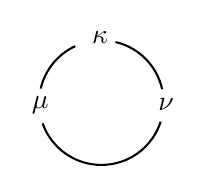
\begin{tikzpicture}[x=0.75pt,y=0.75pt,yscale=-1,xscale=1]
%uncomment if require: \path (0,300); %set diagram left start at 0, and has height of 300

%Shape: Arc [id:dp8573329338560272] 
\draw  [draw opacity=0] (98.78,133.18) .. controls (100.89,124.11) and (107.11,116.62) .. (115.38,112.78) -- (128,140) -- cycle ; \draw   (98.78,133.18) .. controls (100.89,124.11) and (107.11,116.62) .. (115.38,112.78) ;  
%Shape: Arc [id:dp09032135315352707] 
\draw  [draw opacity=0] (156.58,149.13) .. controls (152.72,161.24) and (141.38,170) .. (128,170) .. controls (114.94,170) and (103.83,161.66) .. (99.71,150.01) -- (128,140) -- cycle ; \draw   (156.58,149.13) .. controls (152.72,161.24) and (141.38,170) .. (128,170) .. controls (114.94,170) and (103.83,161.66) .. (99.71,150.01) ;  
%Shape: Arc [id:dp4551353421492913] 
\draw  [draw opacity=0] (134.82,110.78) .. controls (146.02,113.38) and (154.82,122.26) .. (157.3,133.52) -- (128,140) -- cycle ; \draw   (134.82,110.78) .. controls (146.02,113.38) and (154.82,122.26) .. (157.3,133.52) ;  

% Text Node
\draw (93,135.37) node [anchor=north west][inner sep=0.75pt]    {$\mu $};
% Text Node
\draw (154,136.37) node [anchor=north west][inner sep=0.75pt]    {$\nu $};
% Text Node
\draw (122,104.37) node [anchor=north west][inner sep=0.75pt]    {$\kappa $};


\end{tikzpicture}
\end{figure}
\noindent
We now use a cyclic permutation of $\mu, \kappa, \nu $ to obtain the following two equations\footnote{$\lambda$ is summed over in the expression, so we do not consider it in permutation}:
\begin{align*}
    \tensor{\Gamma}{^\lambda _{ \mu \nu}}g_{\kappa \lambda} +\tensor{\Gamma}{^\lambda _{\kappa \nu }}g_{\lambda \mu} &= \partial_\nu g_{\mu\kappa}\\
    \tensor{\Gamma}{^\lambda _{\nu \kappa }}g_{\lambda\mu} +\tensor{\Gamma}{^\lambda _{ \mu \kappa}}g_{\lambda \nu} &= \partial_\kappa g_{\nu\mu}
\end{align*}
Let us now add the first and last equations and subtract the middle one:

\begin{align*}
\partial_\kappa g_{\nu\mu}+\partial_\mu g_{\kappa\nu}- \partial_\nu g_{\mu\kappa}=    \cancel{ \mathcolor{red}{\tensor{\Gamma}{^\lambda _{\nu \kappa }}g_{\lambda\mu}}} +\tensor{\Gamma}{^\lambda _{ \mu \kappa}}g_{\lambda\nu} +\tensor{\Gamma}{^\lambda _{\kappa \mu}}g_{\lambda\nu} +\mathcolor{OliveGreen}{\cancel{\tensor{\Gamma}{^\lambda _{\nu \mu}}g_{\lambda \kappa}}-\cancel{\tensor{\Gamma}{^\lambda _{ \mu \nu}}g_{\lambda\kappa}}} -\cancel{\mathcolor{red}{\tensor{\Gamma}{^\lambda _{\kappa \nu }}g_{\lambda\mu}}}
\end{align*}
We had assumed a torsion-free space and hence the affine connections commute in their lower indices. Hence those terms get cancelled and we finally have the expression as: 
$$\tensor{\Gamma}{^\lambda _{ \mu \kappa}}g_{\lambda\nu} = \frac{1}{2}\brac{\partial_\kappa g_{\nu\mu}+\partial_\mu g_{\kappa\nu}- \partial_\nu g_{\mu\kappa}}$$
Multiply the above by $g^{\nu\alpha}$, then we have: 
\begin{align*}
&\tensor{\Gamma}{^\lambda _{ \mu \kappa}}g_{\lambda\nu} = \frac{1}{2}\brac{\partial_\kappa g_{\nu\mu}+\partial_\mu g_{\kappa\nu}- \partial_\nu g_{\mu\kappa}}\\
\implies &\tensor{\Gamma}{^\lambda _{ \mu \kappa}}g_{\lambda\nu}g^{\nu\alpha} = \frac{1}{2}g^{\nu\alpha}\brac{\partial_\kappa g_{\nu\mu}+\partial_\mu g_{\kappa\nu}- \partial_\nu g_{\mu\kappa}}\\
\implies &\tensor{\Gamma}{^\lambda _{ \mu \kappa}}\tensor{\delta}{^\alpha _\lambda} = \frac{1}{2}g^{\nu\alpha}\brac{\partial_\kappa g_{\nu\mu}+\partial_\mu g_{\kappa\nu}- \partial_\nu g_{\mu\kappa}}\\
\implies &\tensor{\Gamma}{^\alpha _{ \mu \kappa}} = \frac{1}{2}g^{\nu\alpha}\brac{\partial_\kappa g_{\nu\mu}+\partial_\mu g_{\kappa\nu}- \partial_\nu g_{\mu\kappa}}
\end{align*}
Whew!!\emoji{relieved-face} Let us now see an example to find the connection coefficient for 2D polar coordinates.The metric and inverse metric tensor are: 
$$g_{ij} \equiv \begin{pmatrix}
    1 & 0 \\
    0 & r^2
\end{pmatrix}\quad \quad   g^{ij} \equiv \begin{pmatrix}
    1 & 0 \\
    0 & \frac{1}{r^2}
\end{pmatrix}$$
Then taking the derivative of the metric tensor, we have: 
$$\partial_r g_{ij} \equiv \begin{pmatrix}
    1 & 0 \\
    0 & 2r
\end{pmatrix}\quad \quad   \partial_\theta g_{ij} \equiv \begin{pmatrix}
    0 & 0 \\
    0 & 0
\end{pmatrix}$$
The only non-zero element is at $\partial_r g_{\theta \theta}$. Then we only have two non-zero connection coefficients:
\begin{minipage}[t]{0.48\textwidth}
\begin{align*}
\tensor{\Gamma}{^\theta _{r\theta}} &= \frac{1}{2}g^{\theta \theta}\left(\cancel{\partial_\theta g_{\theta r}} + \partial_r g_{\theta \theta} - \cancel{\partial_\theta g_{r \theta}}\right) \\
&= \frac{1}{2r^2} \cdot 2r \\
&= \frac{1}{r}
\end{align*}
\end{minipage}
\hfill
\begin{minipage}[t]{0.48\textwidth}
\begin{align*}
\tensor{\Gamma}{^r _{\theta \theta}} &= \frac{1}{2}g^{r r}\left(\cancel{\partial_\theta g_{r \theta}} + \cancel{\partial_\theta g_{\theta r}} - \partial_r g_{\theta \theta}\right) \\
&= -\frac{1}{2} \cdot 2r \\
&= -r
\end{align*}
\end{minipage}
\subsection{Curls, divergences and other craps}
\subsubsection{Covariant Divergence}

The `ordinary' gradient that we had written earlier, will be generalised to the covariant derivative. Then we will have the divergence modified as: 
\begin{align*}
    \nabla \cdot \tilde{A}\quad \rightarrow \quad \tensor{A}{^\mu _{; \mu}} = \partial_\mu A^\mu + \tensor{\Gamma}{^\mu _{\mu \lambda}}
\end{align*}
From the above relation between metric tensor and the Christoffel symbol, we have:
\begin{align*}
    \tensor{\Gamma}{^\mu _{\mu \lambda}} = \frac{1}{2}g^{\nu \mu}\brac{\partial_\lambda g_{\nu \mu}+\partial_\mu g_{\lambda \nu}-\partial_\nu g_{\mu \lambda}} = \frac{1}{2}\brac{{g^{\nu \mu}\partial_\lambda g_{\nu \mu}}+\mathcolor{blue}{g^{\nu \mu}\partial_\mu g_{\lambda \nu}}-\mathcolor{red}{g^{\nu \mu}\partial_\nu g_{\mu \lambda}}}
\end{align*}
Notice the two coloured terms. Since $\mu$ and $\nu$ are being summed over, we can just interchange them in the, say, red term. Then we will have that both the terms cancel. Thus, we have a simplified expression for the contracted Christoffel symbol as $\tensor{\Gamma}{^\mu _{\mu \lambda}} = \frac{1}{2}g^{\nu \mu}\brac{\partial_\lambda g_{\nu \mu}}$. We will now show that this expression can be reduced to the expression:
$$\tensor{\Gamma}{^\mu _{\mu \lambda}} = \frac{1}{\sqrt{|g|}}\partial_\lambda \brac{\sqrt{|g|}}$$
% $$\tensor{A}{}$$
For that we prove some basic identities:
\begin{identity}
    For any (diagonalisable) matrix $M$, we have:
    $$\Tr (M^{-1}\partial_\lambda M) = \partial_\lambda \ln |M|$$
\end{identity}
\textit{Proof}. Let us calculate the variation of the quantity in the right hand side due to some variation $\delta x^\lambda$ in $x^\lambda$:
\begin{align*}
    \delta \ln |M| &= \ln |M+\delta M| - \ln |M| \\
    &= \ln \brac{\frac{|M+\delta M|}{|M|}} \\
    &= \ln \brac{|M^{-1}||M+\delta M|}\\
    &=\ln \brac{|M^{-1}M + M^{-1}\delta M|}\\
    &=\ln \brac{|\mathds{1}+  M^{-1}\delta M|}
\end{align*}
We now prove another small identity:
$$\ln |M| = \Tr \ln (M)$$
Since M is diagonalisable, we can write the following and then proceed:
\begin{align*}
M &= P D P^{-1}  \\
\Rightarrow \det M &= \det(P D P^{-1}) = \det(D) = \prod_i \lambda_i \\
\Rightarrow \ln \det M &= \ln \left( \prod_i \lambda_i \right) = \sum_i \ln \lambda_i \\
&= \Tr \left( \begin{bmatrix}
\ln \lambda_1 & & \\
& \ln \lambda_2 & \\
& & \ddots
\end{bmatrix} \right) \\
&= \Tr(P^{-1} P \begin{bmatrix}
\ln \lambda_1 & & \\
& \ln \lambda_2 & \\
& & \ddots
\end{bmatrix}) \\
&= \Tr(P \begin{bmatrix}
\ln \lambda_1 & & \\
& \ln \lambda_2 & \\
& & \ddots
\end{bmatrix} P^{-1}) \\
&= \Tr(\ln M)
\end{align*}
So using this identity in the previous result, we have:
\begin{align*}
    \ln \brac{|\mathds{1}+  M^{-1}\delta M|} &= \Tr\ln (\mathds{1}+  M^{-1}\delta M)\\
    &= \Tr\brac{M^{-1}\delta M - \frac{1}{2}{(M^{-1})(\delta M)(M^{-1})(\delta M)}+\ldots}\\
    &=  \Tr M^{-1}\times \delta M  + \ldots
\end{align*}
We somewhat proved this identity\footnote{This derivation is given in Weinberg's book of Cosmology and Gravitation}. Now, we take the case when $M= g$, then we get:
\begin{align*}
   \partial_\lambda \ln |g| =  \Tr(g^{-1}\partial_\lambda g) =\tensor{{\brac{g^{-1}\partial_\lambda g}}}{^\rho _\rho}= \tensor{{g}}{^\rho ^\sigma}\partial_\lambda \tensor{g}{_\sigma _\rho}=2\tensor{\Gamma}{^\mu _\mu _\lambda}
\end{align*}
Thus we get:
$$\tensor{\Gamma}{^\mu _\mu _\lambda} = \frac{1}{2}\partial_\lambda \ln |g|= \frac{1}{2|g|}\partial_\lambda |g|= \frac{1}{\sqrt{|g|}}\partial_\lambda \brac{\sqrt{|g|}}$$
Then we have a cute expression for the covariant divergence:
$$\tensor{A}{^\mu _{; \mu}} = \partial_\mu A^\mu + \frac{1}{\sqrt{|g|}}\partial_\lambda \brac{\sqrt{|g|}}A^\lambda$$
We are not done yet, we can make it even cuter...using the product rule, we have:
$$\partial_\lambda (\sqrt{|g|}A^\lambda) =\sqrt{|g|} \partial_\lambda (A^\lambda)+ \partial_\lambda (\sqrt{|g|}) $$
Substituting this in the above expression, we get: 
$$\tensor{A}{^\mu _{; \mu}} =  \frac{1}{\sqrt{|g|}}\partial_\mu \brac{\sqrt{|g|}A^\mu}$$
Let us check for the spherical polar coordinates where we had seen $g \equiv \mathrm{diag}(1, r^2, r^2\sin\theta) \implies \sqrt{|g|} = r^2 \sin\theta$. Then we will have:
\begin{align*}
    \tensor{A}{^\mu _{; \mu}} &= \frac{1}{r^2 \sin\theta}\brac{\pdv{(r^2\sin\theta A^1)}{r}+\pdv{(r^2\sin\theta A^2)}{\theta}+\pdv{(r^2\sin\theta A^3)}{\phi}}\\
    &=\frac{1}{r^2 \sin\theta}\brac{\sin\theta \pdv{(A^1r^2)}{r}+r^2\pdv{(A^2\sin\theta )}{\theta}+r^2\sin\theta\pdv{( A^3)}{\phi}}\\
   &= {\frac{1}{r^2} \pdv{(A^1r^2)}{r}+\frac{1}{\sin\theta}\pdv{(A^2\sin\theta )}{\theta}+\pdv{( A^3)}{\phi}}
\end{align*}
Now, note that we had earlier done said something about ordinary vectors and how they relate to contravariant vector: $A^\mu = \frac{\widetilde{A_\mu}}{h_\mu}$ and we had also seen the relation between them in spherical coordinates. Using that we have:
\begin{align*}
    \tensor{A}{^\mu _{; \mu}} &= {\frac{1}{r^2} \pdv{(\widetilde{A}_r r^2)}{r}+\frac{1}{\sin\theta}\pdv{(\frac{\widetilde{A}_\theta}{r}\sin\theta )}{\theta}+\pdv{(\frac{\widetilde{A}_\phi}{r\sin\theta})}{\phi}}\\
    &={\frac{1}{r^2} \pdv{(\widetilde{A}_r r^2)}{r}+\frac{1}{r\sin\theta}\pdv{({\widetilde{A}_\theta}\sin\theta )}{\theta}+\frac{1}{{r\sin\theta}}\pdv{({\widetilde{A}_\phi})}{\phi}}
\end{align*}
Lol, this is the formula for normal divergence in spherical polar coordinates that we had been studying and so this new `cute' formula makes sense! Let us now check for the Laplacian and curl too. 
\subsubsection{Covariant Laplacian}
We calculate the following \footnote{Note that the components of the covariant derivative of a scalar function are just the partial derivatives} for a scalar function $\upphi$:
\begin{align*}
    D_\mu D^\mu \upphi = \frac{1}{\sqrt{|g|}}\partial_\mu \brac{\sqrt{|g|}\partial^\mu \upphi}
\end{align*}
Well, note that $\partial^\mu \upphi = g^{\mu \nu}\partial_\nu$ and since the metric tensor is diagonal in this case, only $g^{rr}=1, g^{\theta\theta}=\frac{1}{r^2}, g^{\phi\phi} = \frac{1}{r^2\sin^2\theta}$ will contribute. We then substitute it in the above:
\begin{align*}
    \frac{1}{\sqrt{|g|}} \partial_\mu \left( \sqrt{|g|} \partial^\mu \upphi \right)
    &= \frac{1}{\sqrt{|g|}} \partial_\mu \left( \sqrt{|g|} g^{\mu \nu} \partial_\nu \upphi \right) \\
    &= \frac{1}{r^2 \sin\theta} 
       \brac{ \pdv{}{r} \left( r^2 \sin\theta \pdv{\upphi}{r} \right)
        + \pdv{}{\theta} \left( r^2 \sin\theta \frac{1}{r^2}\cdot\pdv{\upphi}{\theta} \right)
        + \pdv{}{\phi} \left( r^2  \frac{1}{r^2\sin^2\theta}\cdot\pdv{\upphi}{\phi} \right)}\\
    &=\frac{1}{r^2} \pdv{}{r} \left( r^2  \pdv{\upphi}{r} \right) + \frac{1}{r^2\sin\theta}\pdv{}{\theta} \left(  \sin\theta \pdv{\upphi}{\theta} \right) + \frac{1}{r^2\sin^2\theta}\pdv[2]{\upphi}{\phi}
\end{align*}
Wasn't this nice and simple, to derive the form of the Laplacian which has scared us for so long because it just looked ghastly and seemingly popped out of nowhere? 
\subsubsection{A Thing or Two about Levi-Civita}
Curls and cross-products cannot be done without the mention of Levi-Civita symbol. So, let us see a few things about that thing first. 
We all know the famous $\upepsilon_{ijk}$, let us generalise this to higher number of indices and write it with a tilde. So, what we have is:
$$\widetilde{\upepsilon}_{\mu_1\mu_2\ldots\mu_n} = \begin{cases}
    +1, \text{If } {\mu_1\mu_2\ldots\mu_n} \text{is even permutation of } \{0,1,2,\ldots, (n-1)\} \\
     -1, \text{If } {\mu_1\mu_2\ldots\mu_n} \text{is odd permutation of } \{0,1,2,\ldots, (n-1)\}\\
     +0, \text{otherwise}
\end{cases}$$
We will call this object the Levi-Civita `symbol', specifically, since this is not a tensor. Now note one identity:
\begin{identity}
$$\widetilde{\upepsilon}_{\mu_1'\ldots \mu_n'}\det(M)= \widetilde{\upepsilon}_{\mu_1\ldots \mu_n} \tensor{M}{^{\mu_1} _{\mu_1'}}\tensor{M}{^{\mu_2} _{\mu_2'}}\ldots\tensor{M}{^{\mu_n} _{\mu_n'}}$$
\end{identity}
Now take the matrix $M \equiv \pdv{x}{x'}$, then we have from the above formula:
$$\widetilde{\upepsilon}_{\mu_1'\ldots \mu_n'}\left|\pdv{x}{x'}\right|= \widetilde{\upepsilon}_{\mu_1\ldots \mu_n} \pdv{x^{\mu_1}}{x_{\mu_1'}}\pdv{x^{\mu_2}}{x_{\mu_2'}}\ldots\pdv{x^{\mu_n}}{x_{\mu_n'}}\implies\widetilde{\upepsilon}_{\mu_1'\ldots \mu_n'}=\left|\pdv{x'}{x}\right| \widetilde{\upepsilon}_{\mu_1\ldots \mu_n} \pdv{x^{\mu_1}}{x_{\mu_1'}}\pdv{x^{\mu_2}}{x_{\mu_2'}}\ldots\pdv{x^{\mu_n}}{x_{\mu_n'}} $$
We just took the determinant in the denominator in the right hand side and then took the inverse matrix, since inverse of the determinant of a matrix is the determinant of its inverse. \footnote{By the way, I really like these kind of reciprocal sentences. It's a cool thing about mathematics! Another example may be, like sum of trace is the trace of sum.}However, note that the matrix is just the Jacobian and hence the Levi-Civita symbol is a \textit{tensor density} of weight $+1$. Now, also remember that we had previously seen:
$$\mathrm{J} = \sqrt{\frac{|g|}{|g'|}}$$
Then, we will have:
$$\widetilde{\upepsilon}_{\mu_1'\ldots \mu_n'}= \sqrt{\frac{|g|}{|g'|}} \widetilde{\upepsilon}_{\mu_1\ldots \mu_n} \pdv{x^{\mu_1}}{x_{\mu_1'}}\pdv{x^{\mu_2}}{x_{\mu_2'}}\ldots\pdv{x^{\mu_n}}{x_{\mu_n'}}\implies \sqrt{{|g'|}}\widetilde{\upepsilon}_{\mu_1'\ldots \mu_n'}= \sqrt{{|g|}} \widetilde{\upepsilon}_{\mu_1\ldots \mu_n} \pdv{x^{\mu_1}}{x_{\mu_1'}}\pdv{x^{\mu_2}}{x_{\mu_2'}}\ldots\pdv{x^{\mu_n}}{x_{\mu_n'}} $$
Thus the quantity ${\upepsilon}_{\mu_1\ldots\mu_n} = \sqrt{|g|}\widetilde{\upepsilon}_{\mu_1\ldots\mu_n}$ transforms as a tensor and we can do all the up and down game with the indices. This we call as \textbf{Levi-Civita tensor}. We also sometimes define the Levi-Civita symbol as $\widetilde{\upepsilon}^{\mu_1'\ldots \mu_n'}$ which is of weight $-1$\footnote{This is numerically equal to $\mathrm{sgn}(g) \widetilde{\upepsilon}_{\mu_1\ldots\mu_n}$} and then we get ${\upepsilon}^{\mu_1\ldots\mu_n} = \frac{1}{\sqrt{|g|}}\widetilde{\upepsilon}^{\mu_1\ldots\mu_n}$.\\[0.3cm]
Most of the time, we contract some of the indices of the Levi-Civita tensor and we obtain some Kronecker deltas. We have an identity for contracting $p$ such indices: 
$$\epsilon^{\mu_1 \mu_2 \cdots \mu_p \alpha_1 \cdots \alpha_{n-p}} 
\epsilon_{\mu_1 \mu_2 \cdots \mu_p \beta_1 \cdots \beta_{n-p}} 
= (-1)^s\, p!(n - p)! \, \delta^{[\alpha_1\ldots \alpha_{n-p}]}_{\beta_1\ldots \beta_{n-p}}$$
Now, wtf does the right hand side denote? Here $s$ is the number of negative eigenvalues of the metric tensor but what about the weird delta symbol? Carroll writes it as an anti-symmetrised product of Kronecker deltas. We elaborate it a bit further. For any tensor $T$, the notation $\tensor{T}{^{[\mu_1\ldots\mu_n]}}$ is equal to: 
$$\tensor{T}{^{[\mu_1\ldots\mu_n]}} = \frac{1}{n!}\sum\limits_{\pi \in S_n}\mathrm{sgn}(\pi)\tensor{T}{^{\mu_{\pi(1)}\mu_{\pi(2)}\ldots\mu_{\pi(n)}}}$$
Well, did I make it more complicated? Perhaps, but complications lead to clarifications. $S_n$ is the permutation group of order $n$, $\mathrm{sgn}(\pi)$ denotes the sign of the permutation and is positive if it is obtained from even number of exchanges and negative otherwise. Let us see for $S_3$, the group is then:
$$S_3\equiv  \{\underbrace{\{1,2,3\}}_{\pi_1},\underbrace{\{1,3,2\}}_{\pi_2},\underbrace{\{2,1,3\}}_{\pi_3},\underbrace{\{2,3,1\}}_{\pi_4},\underbrace{\{3,1,2\}}_{\pi_5},\underbrace{\{3,2,1\}}_{\pi_6} \}$$
Then we can check that we have $\mathrm{sgn}(\pi_i) = +1$ for $i=1,4,5$ and $-1$ for $i=2,3,6$
So, similarly the Kronecker delta can be written as: 
$$\tensor{\delta}{^{[\alpha_1\ldots\alpha_{n-p}]} _{\beta_1\ldots\beta_{n-p}}} = \frac{1}{(n-p)!}\sum\limits_{\pi \in S_n}\mathrm{sgn}(\pi) \prod\limits_i \tensor{\delta}{^{\alpha_{\pi(i)}} _{\beta(i)}}$$
And now using Leibniz's formula for determinant\footnote{The formula says that for any matrix A, we have:
$$\det(A) = \sum_{\tau \in S_n} \operatorname{sgn}(\tau) \prod_{i=1}^{n} a^{i}_{\tau(i)} 
= \sum_{\sigma \in S_n} \operatorname{sgn}(\sigma) \prod_{i=1}^{n} a_{\sigma(i)}^{i}$$
}, we have: 
$$\tensor{\delta}{^{[\alpha_1\ldots\alpha_{n-p}]} _{\beta_1\ldots\beta_{n-p}}} = \frac{1}{(n-p)!}\det(\mathrm{\delta})$$
where, $$\delta \equiv 
\begin{pmatrix}
\delta^{\alpha_1}_{\beta_1} & \cdots & \delta^{\alpha_{n-p}}_{\beta_1} \\
\vdots & \ddots & \vdots \\
\delta^{\alpha_1}_{\beta_{n-p}} & \cdots & \delta^{\alpha_{n-p}}_{\beta_{n-p}}
\end{pmatrix}$$
Then the final expression that we have is: 
$$\epsilon^{\mu_1 \mu_2 \cdots \mu_p \alpha_1 \cdots \alpha_{n-p}} 
\epsilon_{\mu_1 \mu_2 \cdots \mu_p \beta_1 \cdots \beta_{n-p}} 
= (-1)^s p! \det{\delta}$$
Well, let us see one example, for this that we know. For this, we take $p=1$ and $n=3$, then $n-p = 2$. So, we have:
$$\epsilon^{ijk}\epsilon{ilm} = (-1)^s \times 1! \times \det\begin{pmatrix}
    \delta^j_l &  \delta^k_l \\
     \delta^j_m &  \delta^k_m
\end{pmatrix} = (-1)^s \brac{\delta^j_l \delta^k_m - \delta^j_m \delta^k_l}$$
Isn't this fun to finally see how this expression comes? Well, for me, yes but it is just an amusement for me, 'coz ultimately, to use it, we have to kinda remember it. Deriving things from scratch is a painful patch, with time to lose and little to match. 
\subsubsection{Covariant Curl}



